%%%%%%%%%%%%%%%%%%%%%%%%%%%%%%%%%%%%%%%%%
% University/School Laboratory Report
% LaTeX Template
% Version 3.1 (25/3/14)
%
% This template has been downloaded from:
% http://www.LaTeXTemplates.com
%
% Original author:
% Linux and Unix Users Group at Virginia Tech Wiki 
% (https://vtluug.org/wiki/Example_LaTeX_chem_lab_report)
%
% License:
% CC BY-NC-SA 3.0 (http://creativecommons.org/licenses/by-nc-sa/3.0/)
%
%%%%%%%%%%%%%%%%%%%%%%%%%%%%%%%%%%%%%%%%%

%----------------------------------------------------------------------------------------
%	PACKAGES AND DOCUMENT CONFIGURATIONS
%----------------------------------------------------------------------------------------

\documentclass{article}

\usepackage[version=3]{mhchem} % Package for chemical equation typesetting
\usepackage{siunitx} % Provides the \SI{}{} and \si{} command for typesetting SI units
\usepackage{graphicx} % Required for the inclusion of images
\usepackage{natbib} % Required to change bibliography style to APA
\usepackage{amsmath} % Required for some math elements 
\usepackage{float}
\usepackage[margin=1in]{geometry}
\usepackage{hyperref}
\usepackage{listings}
\usepackage{xcolor}
\usepackage[british]{babel}
\selectlanguage{british}

\setlength\parindent{0pt} % Removes all indentation from paragraphs

\renewcommand{\labelenumi}{\alph{enumi}.} % Make numbering in the enumerate environment by letter rather than number (e.g. section 6)

%\usepackage{times} % Uncomment to use the Times New Roman font

\definecolor{codeBackground}{rgb}{0.95,0.95,0.95}
\definecolor{codeKeyword}{rgb}{0.75, 0.25, 0.0}
\definecolor{codeComment}{rgb}{0.0, 0.55, 0.45}
\definecolor{codeLineNumbers}{rgb}{0.2, 0.2, 0.2}

\lstdefinestyle{DatasetConfig}{
	backgroundcolor=\color{codeBackground},   
    %commentstyle=\color{codeComment},
    keywordstyle=\color{codeKeyword},
    morekeywords={FILE},
    numbers=left,
    numberstyle=\color{codeLineNumbers},
    %stringstyle=\color{codepurple},
    %basicstyle=\ttfamily\footnotesize,
    %breakatwhitespace=false,         
    %breaklines=true,                 
    %captionpos=b,                    
    %keepspaces=true,                 
    %numbers=left,                    
    %numbersep=5pt,                  
    %showspaces=false,                
    %showstringspaces=false,
    %showtabs=false,                  
    %tabsize=2
}

\lstdefinestyle{CommandLine}{
	backgroundcolor=\color{codeBackground},   
	numbers=none
}

%----------------------------------------------------------------------------------------
%	DOCUMENT INFORMATION
%----------------------------------------------------------------------------------------

\title{Computer Vision - Final Project \\ Tree Detection} % Title

\author{Davide Dravindran Pistilli} % Author name

\date{\today} % Date for the report

\begin{document}

\maketitle % Insert the title, author and date

\section{Introduction}
The purpose of this project is to create a program that is able to detect and locate all major trees in a given image. The process is organised in three main phases:
\begin{itemize}
\item \textbf{segmentation}: the image is segmented to identify the areas that have to be analysed;
\item \textbf{classification}: the most relevant segments are analysed through a Bag of Words vocabulary in order to check the presence or absence of trees;
\item \textbf{growth}: the candidate regions resulting from the previous step are enlarged in order to envelop the entire tree.
\end{itemize}

\section{Training}
\subsection{Dataset}
The Bag of Words approach requires a training phase to be performed to enable detection. This process uses as input a text file that specifies all training images with the trees they contain, if there are any (\textit{Listing \ref{code:dataset}}).

\lstset{style=DatasetConfig}
\lstinputlisting[
	firstline=1, 
	lastline=6, 
	caption={\footnotesize\texttt{dataset2.txt}.},
	captionpos=b, 
	label={code:dataset}
]{../data/dataset2/dataset2.txt}

A rectangle specified by four parameters (x and y coordinates of the top-left corner, the width and the height) is defined for each tree.
The training dataset used for this project contains 246 images, and is available on Google Drive\footnote{\url{https://drive.google.com/file/d/16PJH2uVHWV3S7zXArRMKbwitqt5M1Y9y/view?usp=sharing}}.
All images and the trees chosen for training can be viewed through a python program, \texttt{DatasetVisualiser.py}.

\subsection{Training Program}
The training phase can be run with a command structured as specified below:
\begin{lstlisting}[style=CommandLine]
./Prj train ../dataset2/dataset2.txt ../dataset2/
\end{lstlisting}
where the arguments are as follows:
\begin{itemize}
\item \textbf{train}: special keyword that tells the program to train the Bag of Words data;
\item \textbf{../dataset2/dataset2.txt}: configuration file for the dataset;
\item \textbf{../dataset2/}: root folder for the dataset images.
\end{itemize}

The actual training commences after the configuration file has been parsed.
First of all, the program computes SIFT features from suitable areas of the image. If the image contains one or more trees, features are computed for each one in their respective rectangles. 
If there are no trees, however, features are computed on each node of a quad-tree that has the whole image as root (\textit{Listing \ref{code:imgpyramid}}). 

\lstinputlisting[
	firstline=157, 
	lastline=159, 
	firstnumber=157, 
	language=c++, 
	caption={\footnotesize \texttt{include/utility.hpp}}, 
	captionpos={b}, 
	label={code:imgpyramid}
]{../include/utility.hpp}

A depth of 2 provides an adequate number of views on the image while avoiding very specific details, such as individual forest trees.
Note that all images are resized to a fixed resolution.

Completion of this step yields two distinct sets of features: tree features and non-tree features.
These sets are then separately clustered to produce the corresponding Bag of Words vocabularies.

However, a reference histogram for each class is also required to classify an image. Hence, the final training step reloads each training image (images are loaded only when needed to reduce memory usage) and computes its BoW histograms on the same areas as before, using the appropriate vocabulary.
To avoid using weak areas of the image, a minimum number of features is required for a histogram to be computed and considered in the average (\textit{Listing \ref{code:minTrainFeatures}}).

\lstinputlisting[
	firstline=36, 
	lastline=37, 
	firstnumber=36, 
	language=c++, 
	caption={\footnotesize \texttt{include/TreeDetectorTrainer.hpp}},
	captionpos={b}, 
	label={code:minTrainFeatures}
]{../include/TreeDetectorTrainer.hpp}

At the end of the process, the two vocabularies and the average tree and non-tree histograms are saved to a file named \texttt{trees.xml} in the dataset root folder.

\section{Detection}
\subsection{Start-up}
The detection phase can be run with a command structured as specified below:

\begin{lstlisting}[style=CommandLine]
./Prj detect trees.xml testdata/Figure_1.jpg
\end{lstlisting}

where the arguments are:
\begin{itemize}
\item \textbf{detect}: special keyword that tells the program to detect trees in an image;
\item \textbf{trees.xml}: file containing the trained vocabularies and histograms;
\item \textbf{testdata/Figure\_1.jpg}: image on which detection is performed.
\end{itemize}

After loading the input image, the first step is to resize it to a fixed resolution (\textit{Listing \ref{code:imageResolution}}), as done during training, in order to have a normalised initial condition.

\lstinputlisting[
	firstline=34, 
	lastline=36, 
	firstnumber=34, 
	language=c++, 
	caption={\footnotesize \texttt{include/utility.hpp}},
	captionpos={b}, 
	label={code:imageResolution}
]{../include/utility.hpp}

\subsection{Pre-processing}
To get meaningful results from the BoW classification, relevant areas of the image that will later be analysed must be identified. This is achieved by segmenting the image using the watershed algorithm. All resulting segments pass on to the analysis step.

Two filters are applied before segmenting the image: a bilateral and a Gaussian filter.
The bilateral filter smoothens the image while preserving its edges. The Gaussian filter, then, smoothens the whole image uniformly, further reducing the effect of small high contrast areas (such as leaves).

After these filters have been applied, the actual segmentation can be performed (\textit{Listing \ref{code:imageSegmentation}}).

\lstinputlisting[
	firstline=310, 
	lastline=327, 
	firstnumber=310, 
	language=c++, 
	caption={\footnotesize \texttt{src/Image.cpp}},
	captionpos={b}, 
	label={code:imageSegmentation}
]{../src/Image.cpp}

The watershed algorithm requires a set of starting seeds from which to grow the regions. These should be the farthest points from the edges of the image, so the 'edge map' and then the 'distance transform' are computed.
To obtain only the farthest points from the edges, all values are normalised and a threshold is applied.
Then, each connected component is labelled differently from the others so that watershed considers each of them a separate segment.

Another approach was also attempted: instead of segmenting the image through an algorithm like watershed, fixed segments were used. These were obtained through the same quad-tree structure used for training, just with a higher depth. The overall results were comparable to the current solution and sometimes even better, but the execution time was up to three-fold longer in some cases. Due to this and some difficulties with the growing phase, the quad-tree approach was replaced with watershed.

\subsection{Analysis}
Depending on the image, watershed could output a huge amount of segments. The first analysis step is to choose only those, whose score is high enough to be considered part of a tree.
The score for each segment is computed as shown in \textit{Listing \ref{code:scoreComputation}} based on its distances from the two classes: tree and non-tree.

\lstinputlisting[
	firstline=194, 
	lastline=199, 
	firstnumber=194, 
	language=c++, 
	caption={\footnotesize \texttt{src/TreeDetector.cpp}},
	captionpos={b}, 
	label={code:scoreComputation}
]{../src/TreeDetector.cpp}

These are the distances between the histogram of the segment (computed with the appropriate vocabulary) and the average histogram of the class.
A negative distance means that the segment does not have a sufficient number of features.

The candidate segments are then sorted by decreasing score, and go through a fusion round where overlapping segments are fused together. All resulting candidates move to the growth phase.

\subsection{Growth}
Candidates usually do not envelop the entirety of a tree due to over-segmentation. This is solved by growing each one of them.
For each candidate, all four sides of the rectangle are examined at each iteration, and the best one is chosen for expansion. If no areas are suitable, the growth is stopped, a fusion round is performed and the next candidate is processed.
The results of this phase are the final trees that will be displayed.

This is the most demanding part of the program, since SIFT features are continuously computed and matched against two BoW vocabularies. Without it, however, many trees are detected correctly but become over-segmented with non-overlapping regions.

\section{Results}
\subsection{Benchmark Dataset}
The quality of the results is quite mixed: since trees can appear in many different scenes and illumination conditions, there is no parameter combination that is effective for all images.
The chosen parameters aim at achieving acceptable results across as many settings as possible.

\textit{Figure \ref{img:benchmark1}} shows how clear and isolated trees can be detected, provided that they have enough features. The tree on the left, in fact, had too few features to be considered. Lowering the thresholds further resulted in many false positives and lower quality regions overall.

\begin{figure}[h]
\begin{center}
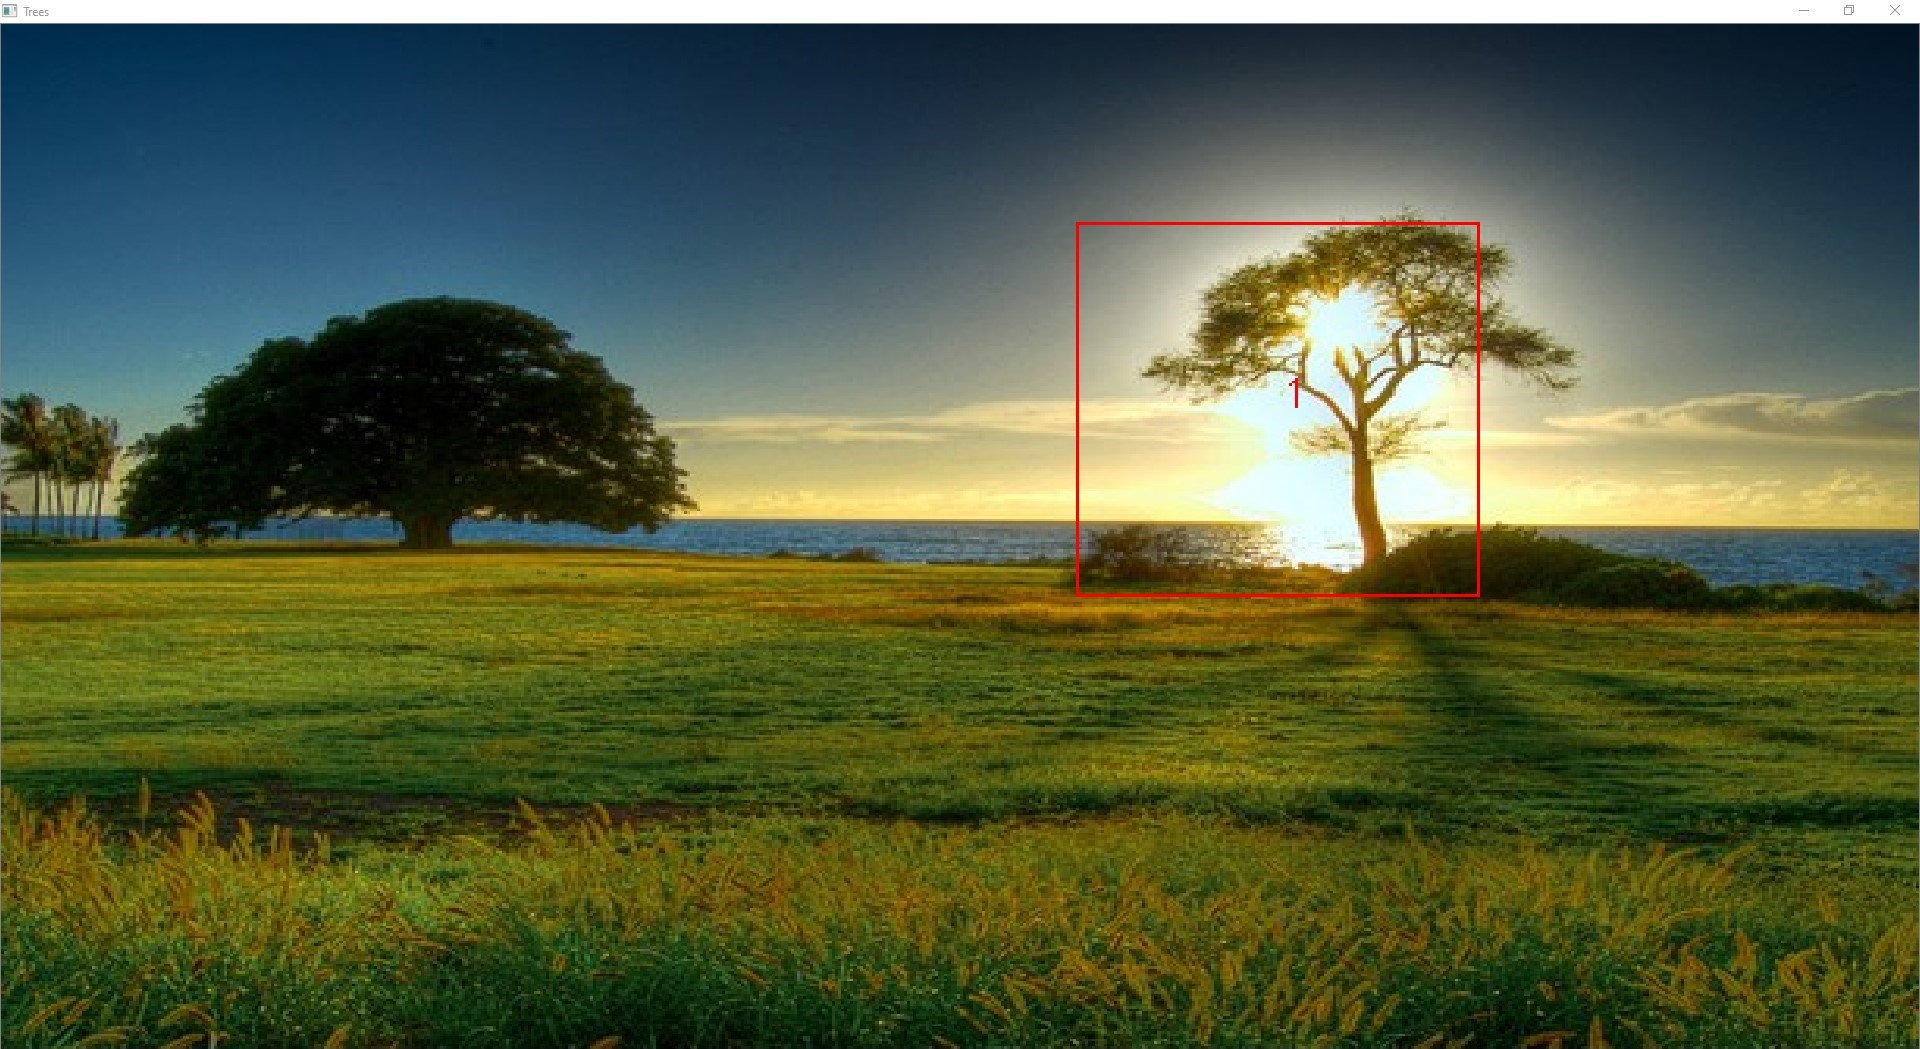
\includegraphics[width=1\textwidth]{images/b1}
\caption{\footnotesize{Figure\_1.jpg}}
\label{img:benchmark1}
\end{center}
\end{figure}

\begin{figure}[h]
\begin{center}
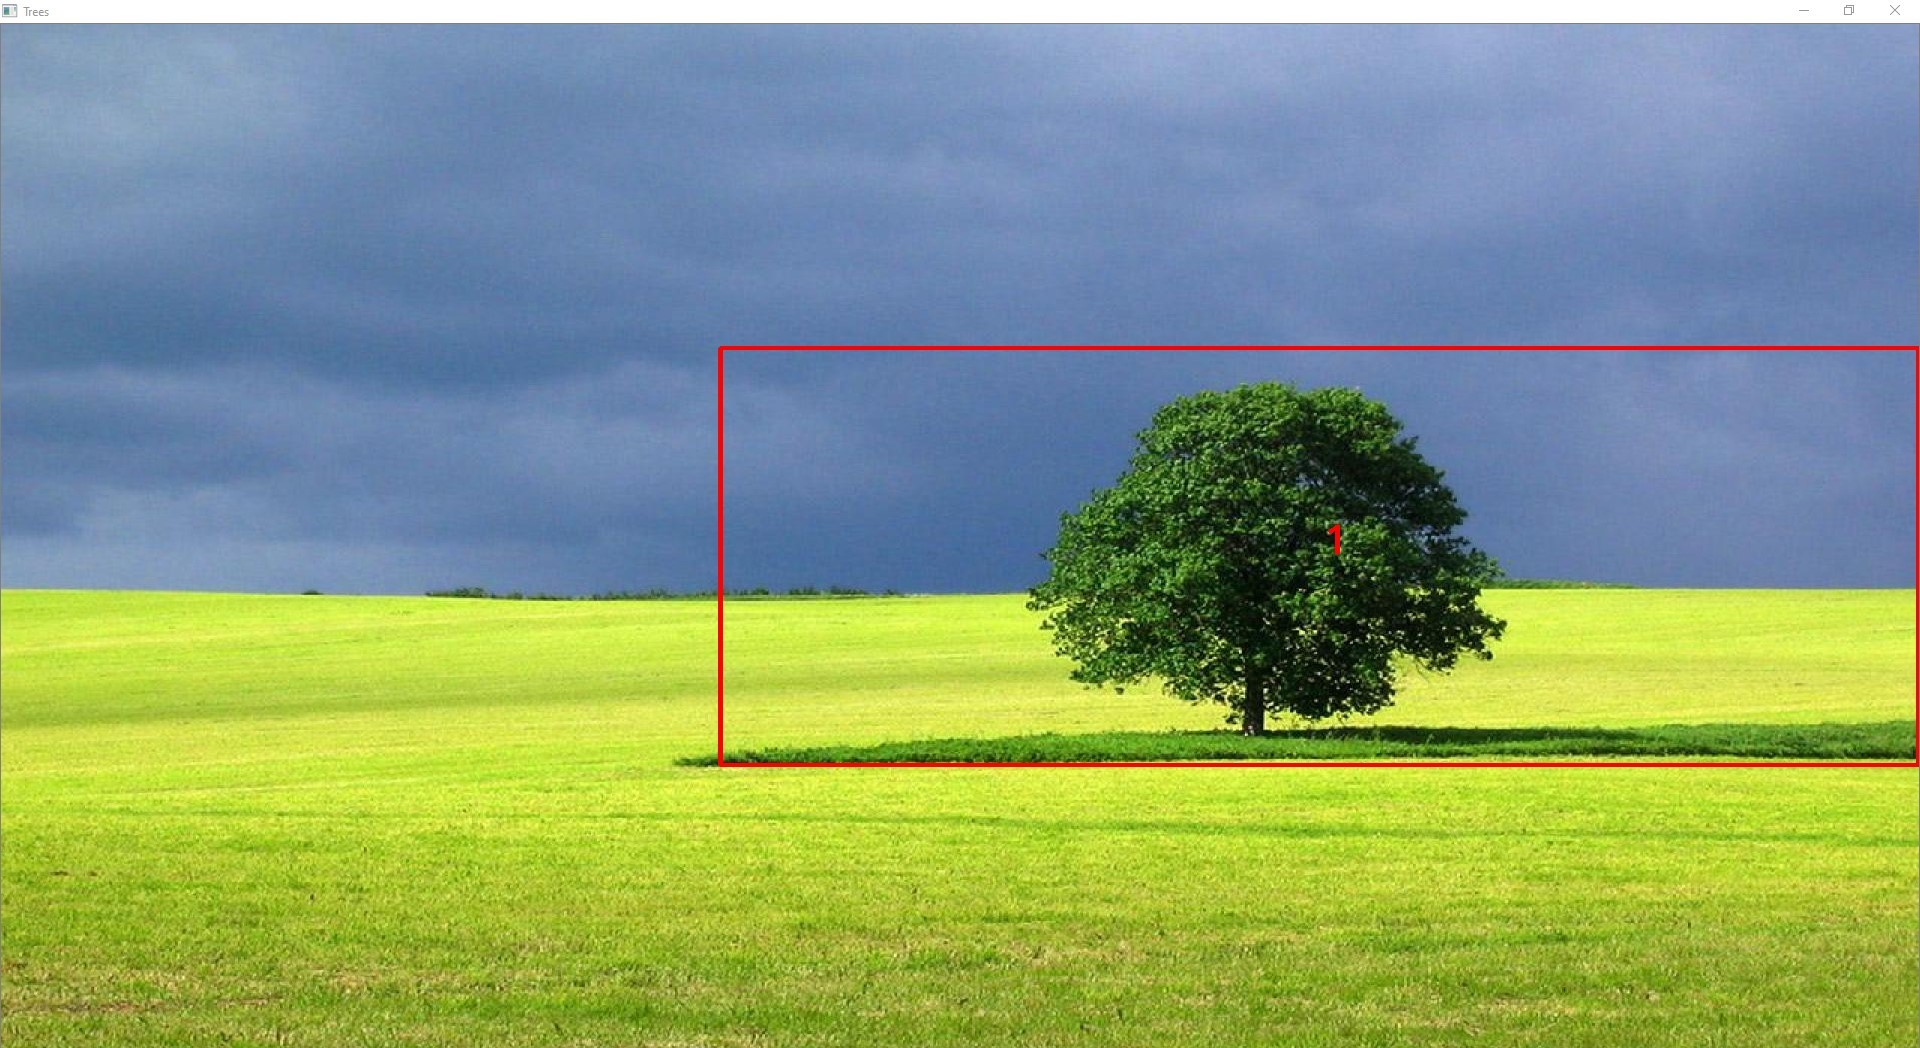
\includegraphics[width=1\textwidth]{images/b2}
\caption{\footnotesize{Figure\_2.jpg}}
\label{img:benchmark2}
\end{center}
\end{figure}

\begin{figure}[h]
\begin{center}
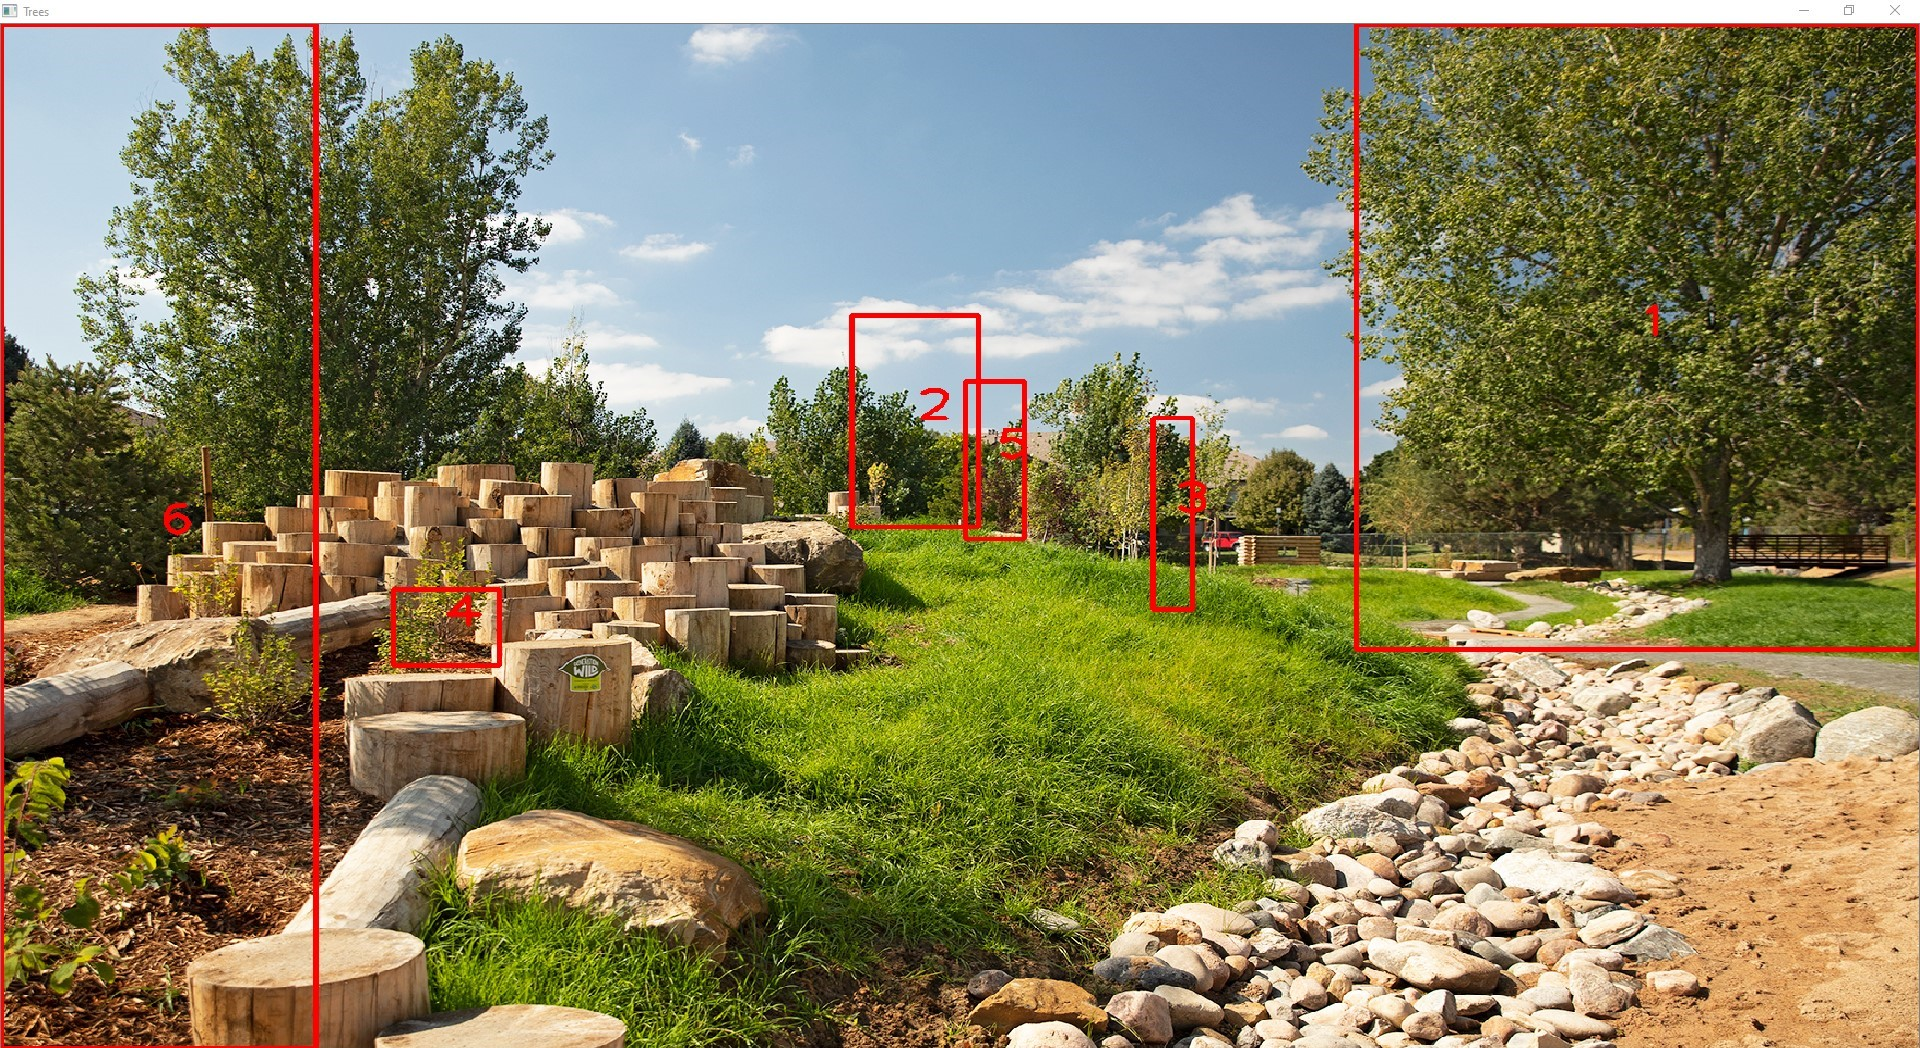
\includegraphics[width=1\textwidth]{images/b3}
\caption{\footnotesize{Figure\_3.jpg}}
\label{img:benchmark3}
\end{center}
\end{figure}

\textit{Figure \ref{img:benchmark3}} shows some false positives that survived the analysis phase due to their high scores (trees from 2 to 5). Tree number 6, however, expanded toward the wrong direction during the growth phase.

\begin{figure}[h]
\begin{center}
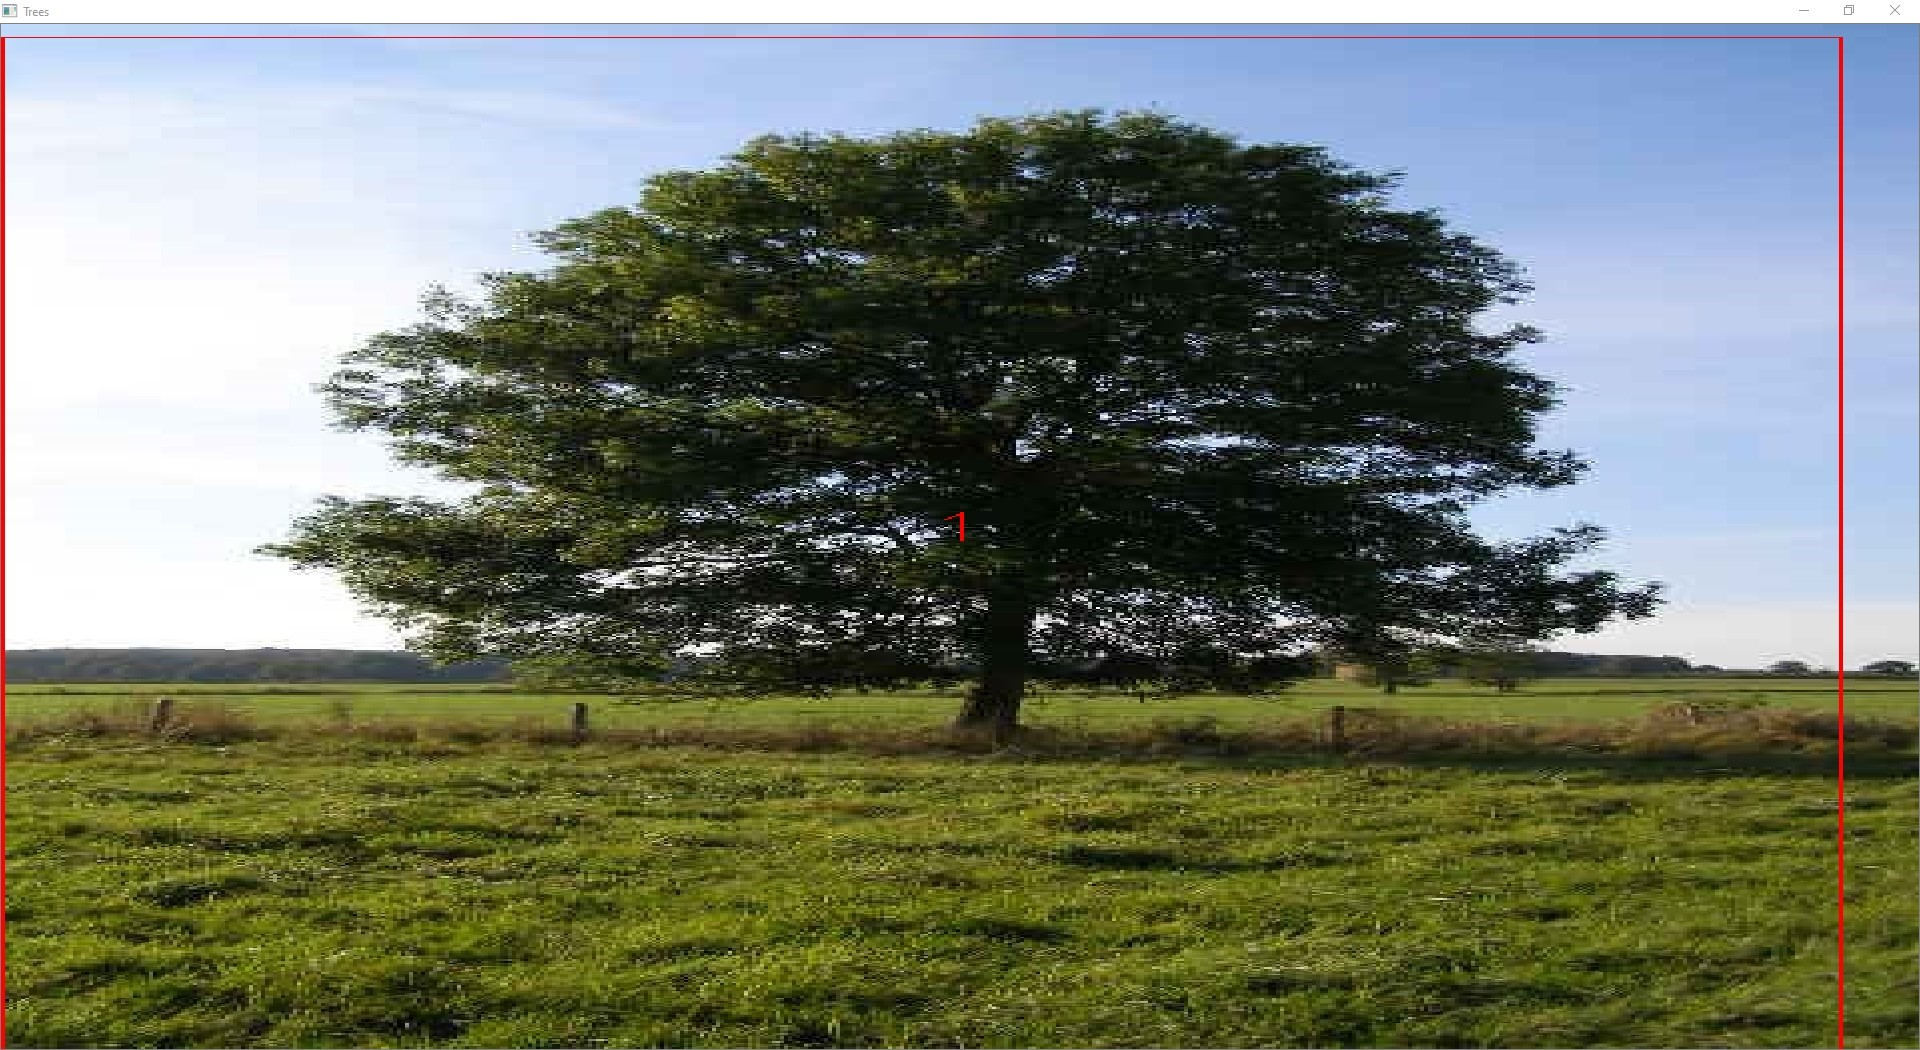
\includegraphics[width=1\textwidth]{images/b4}
\caption{\footnotesize{Figure\_4.jpg}}
\label{img:benchmark4}
\end{center}
\end{figure}

\begin{figure}[h]
\begin{center}
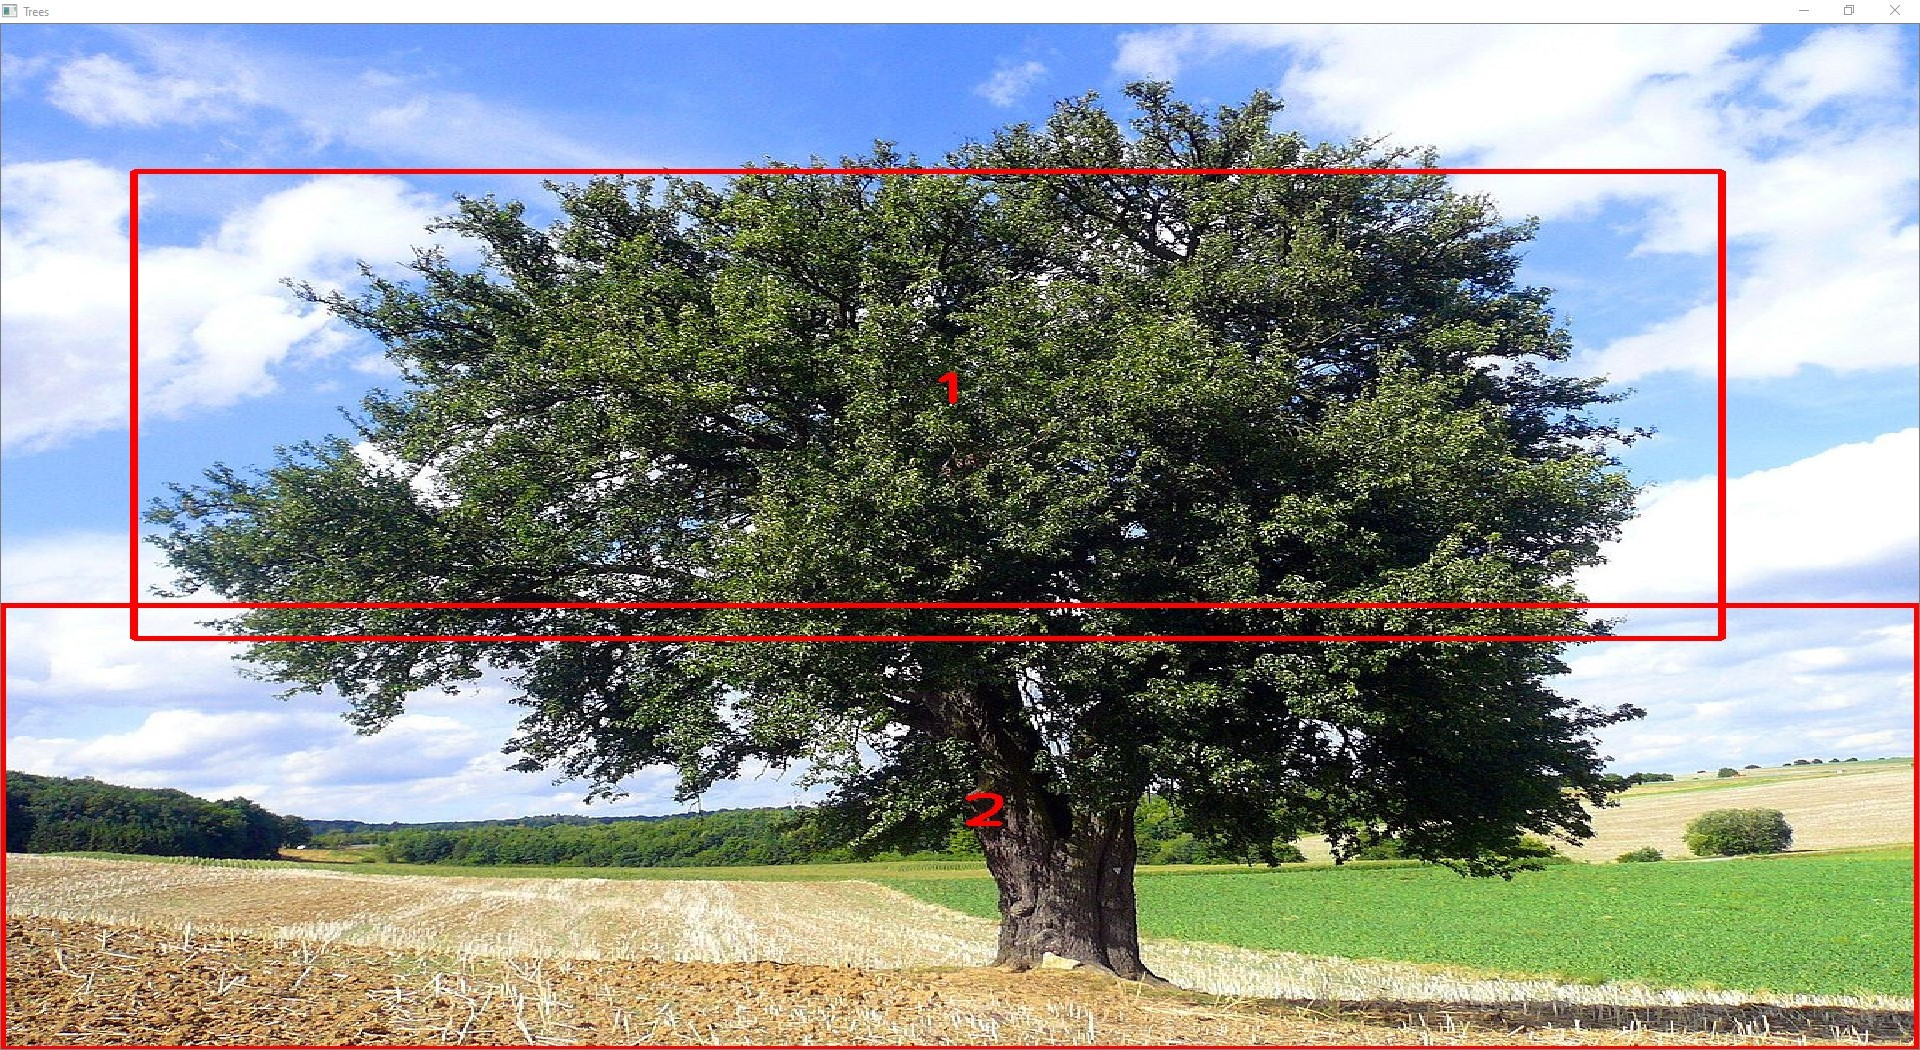
\includegraphics[width=1\textwidth]{images/b5}
\caption{\footnotesize{Figure\_5.jpg}}
\label{img:benchmark5}
\end{center}
\end{figure}

\textit{Figure \ref{img:benchmark5}} illustrates a situation where the growth phase is unable to compensate for the over-segmentation resulting from watershed: growing any of those two regions would have caused an excessive reduction in their score, so the algorithm ended.

\begin{figure}[h]
\begin{center}
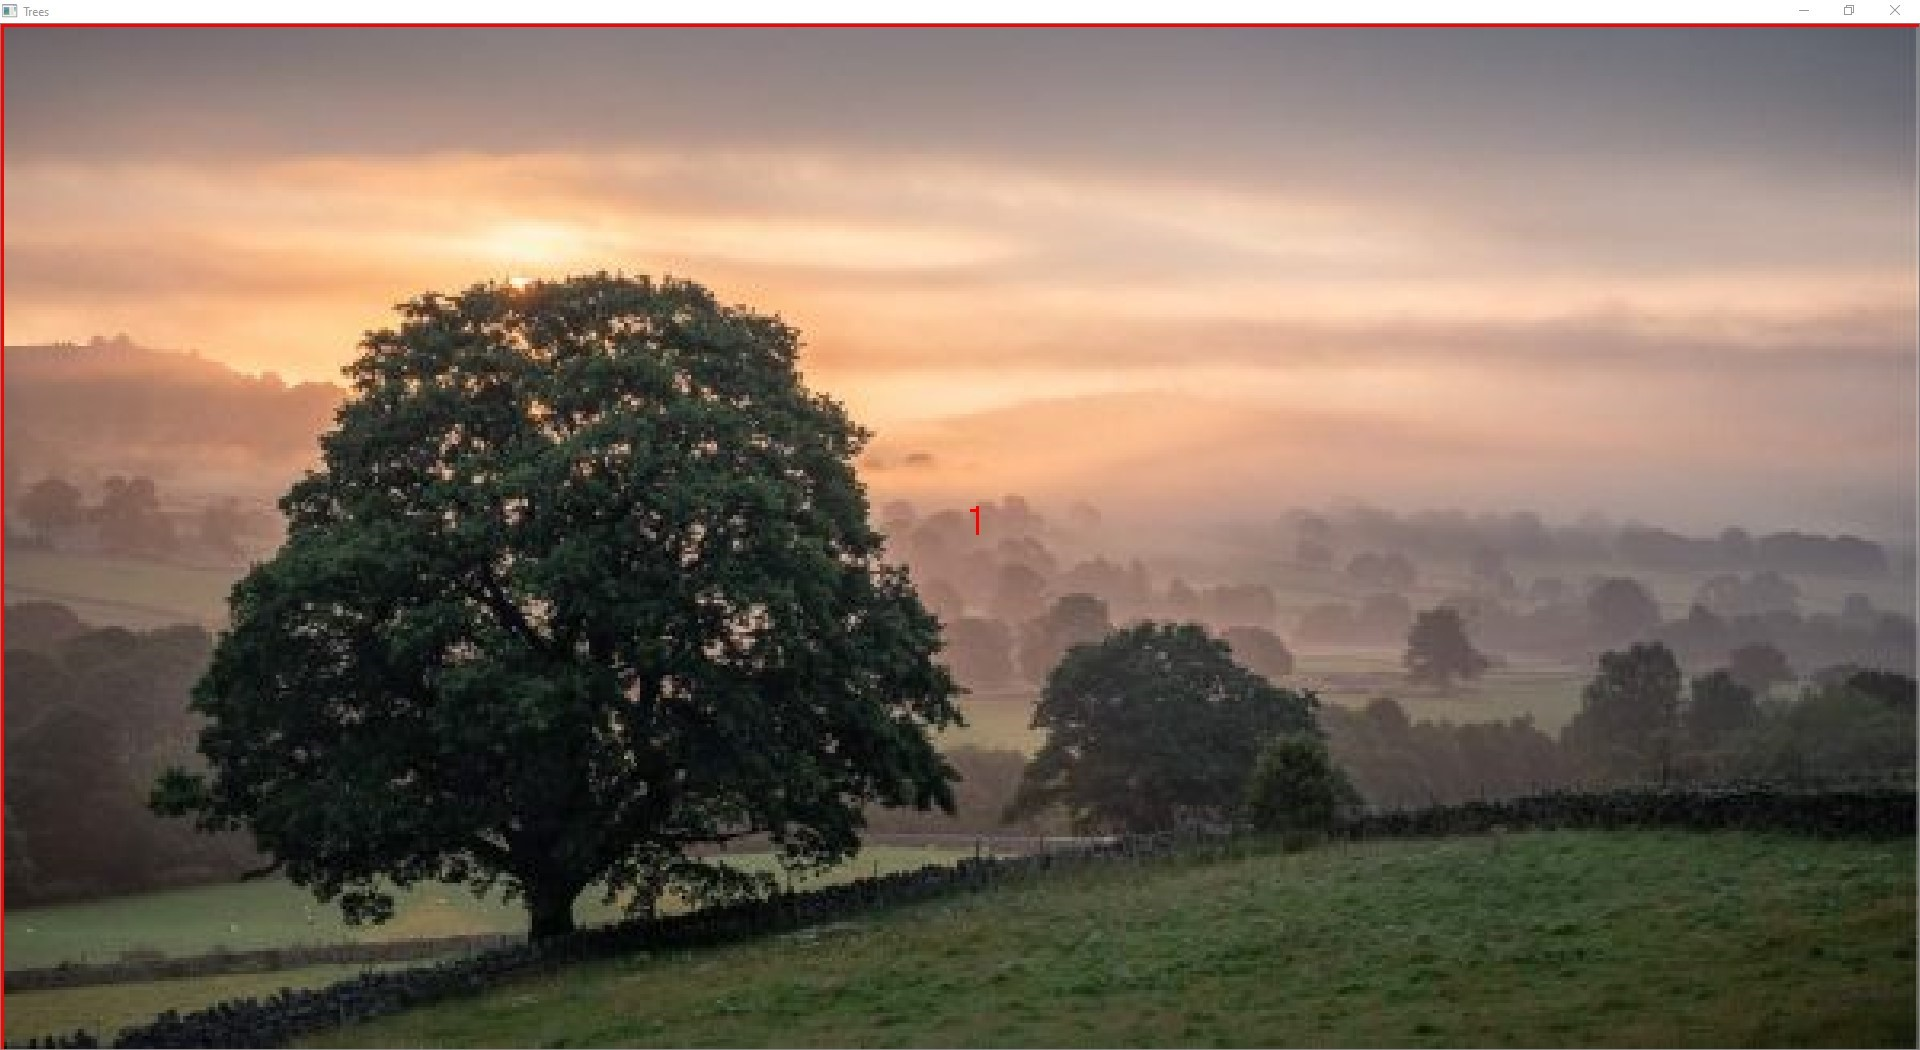
\includegraphics[width=1\textwidth]{images/b6}
\caption{\footnotesize{Figure\_6.jpg}}
\label{img:benchmark6}
\end{center}
\end{figure}

\textit{Figure \ref{img:benchmark6}} is an example where the segmentation phase failed to provide small enough regions, so the entire image was analysed. As with the previous images, parameters could be tuned to enable detection at the expense of overall accuracy in the entire dataset.

\begin{figure}[h]
\begin{center}
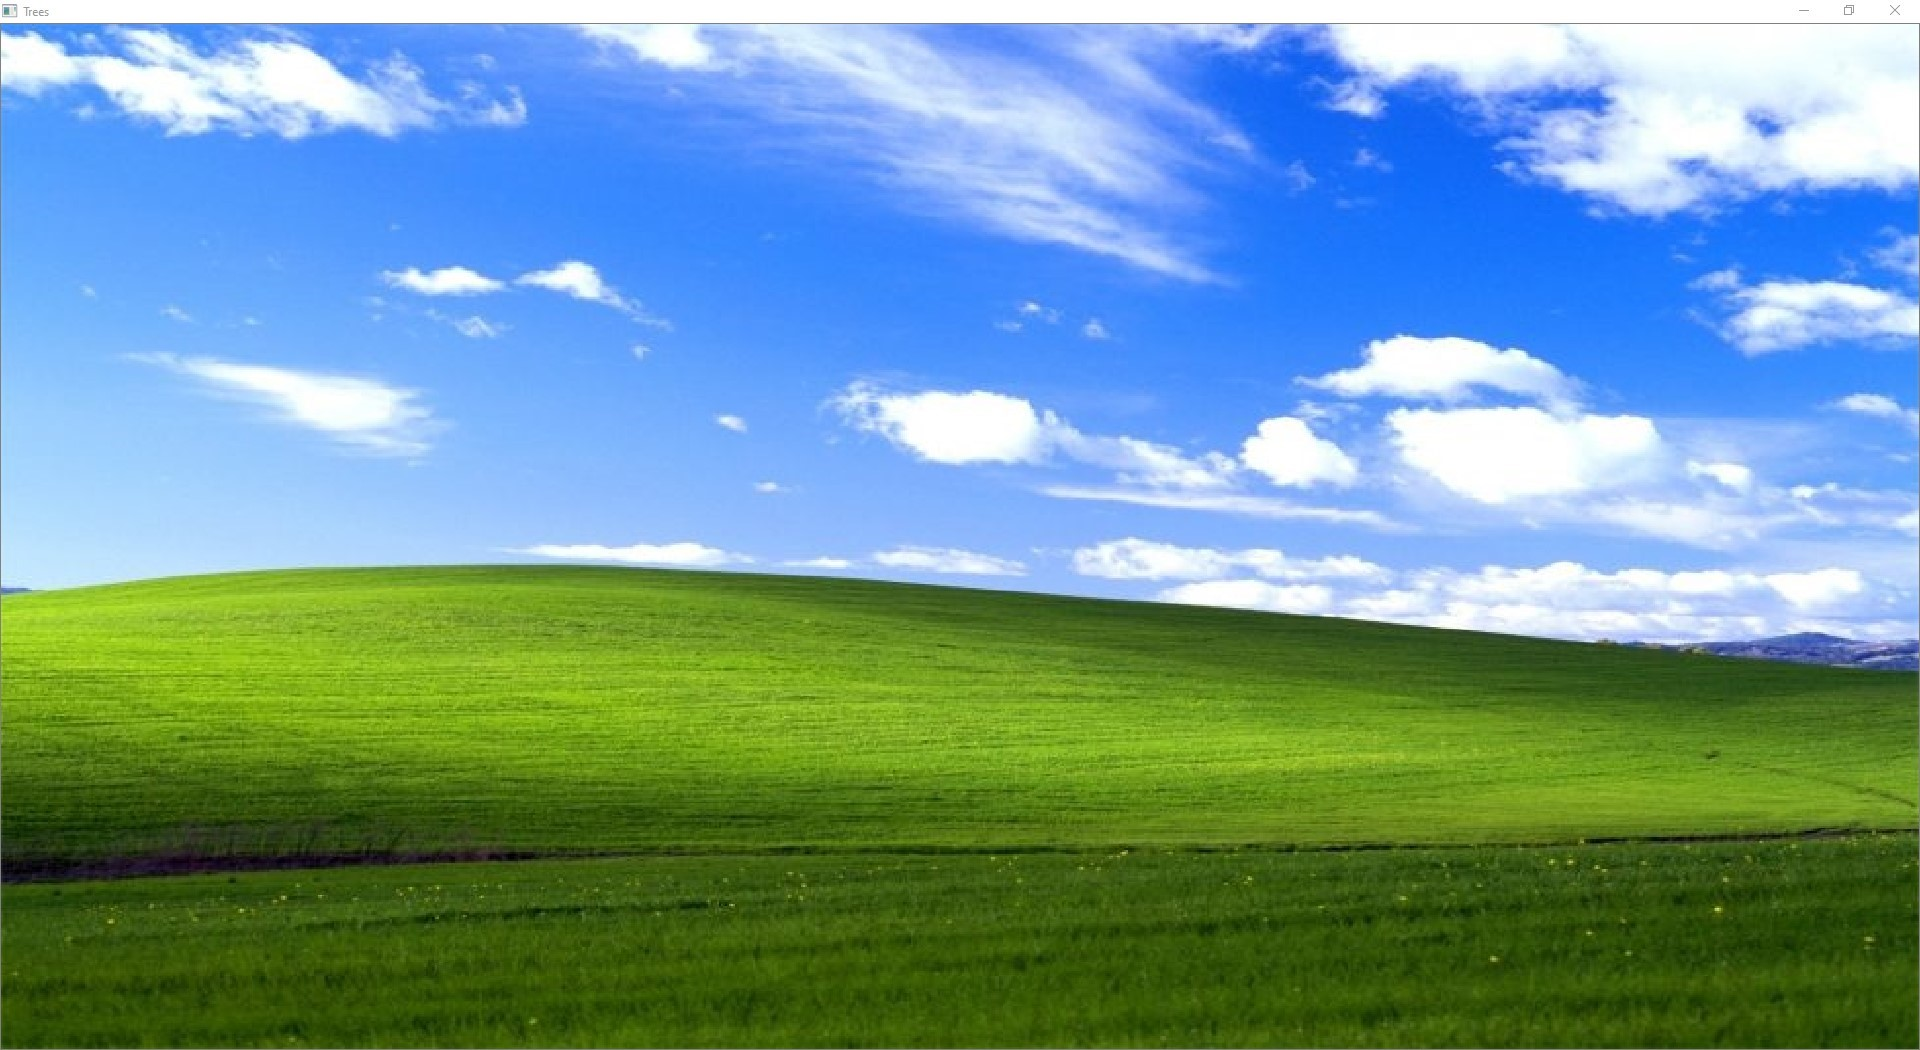
\includegraphics[width=1\textwidth]{images/b7}
\caption{\footnotesize{Figure\_7.jpg}}
\label{img:benchmark7}
\end{center}
\end{figure}

\begin{figure}[h]
\begin{center}
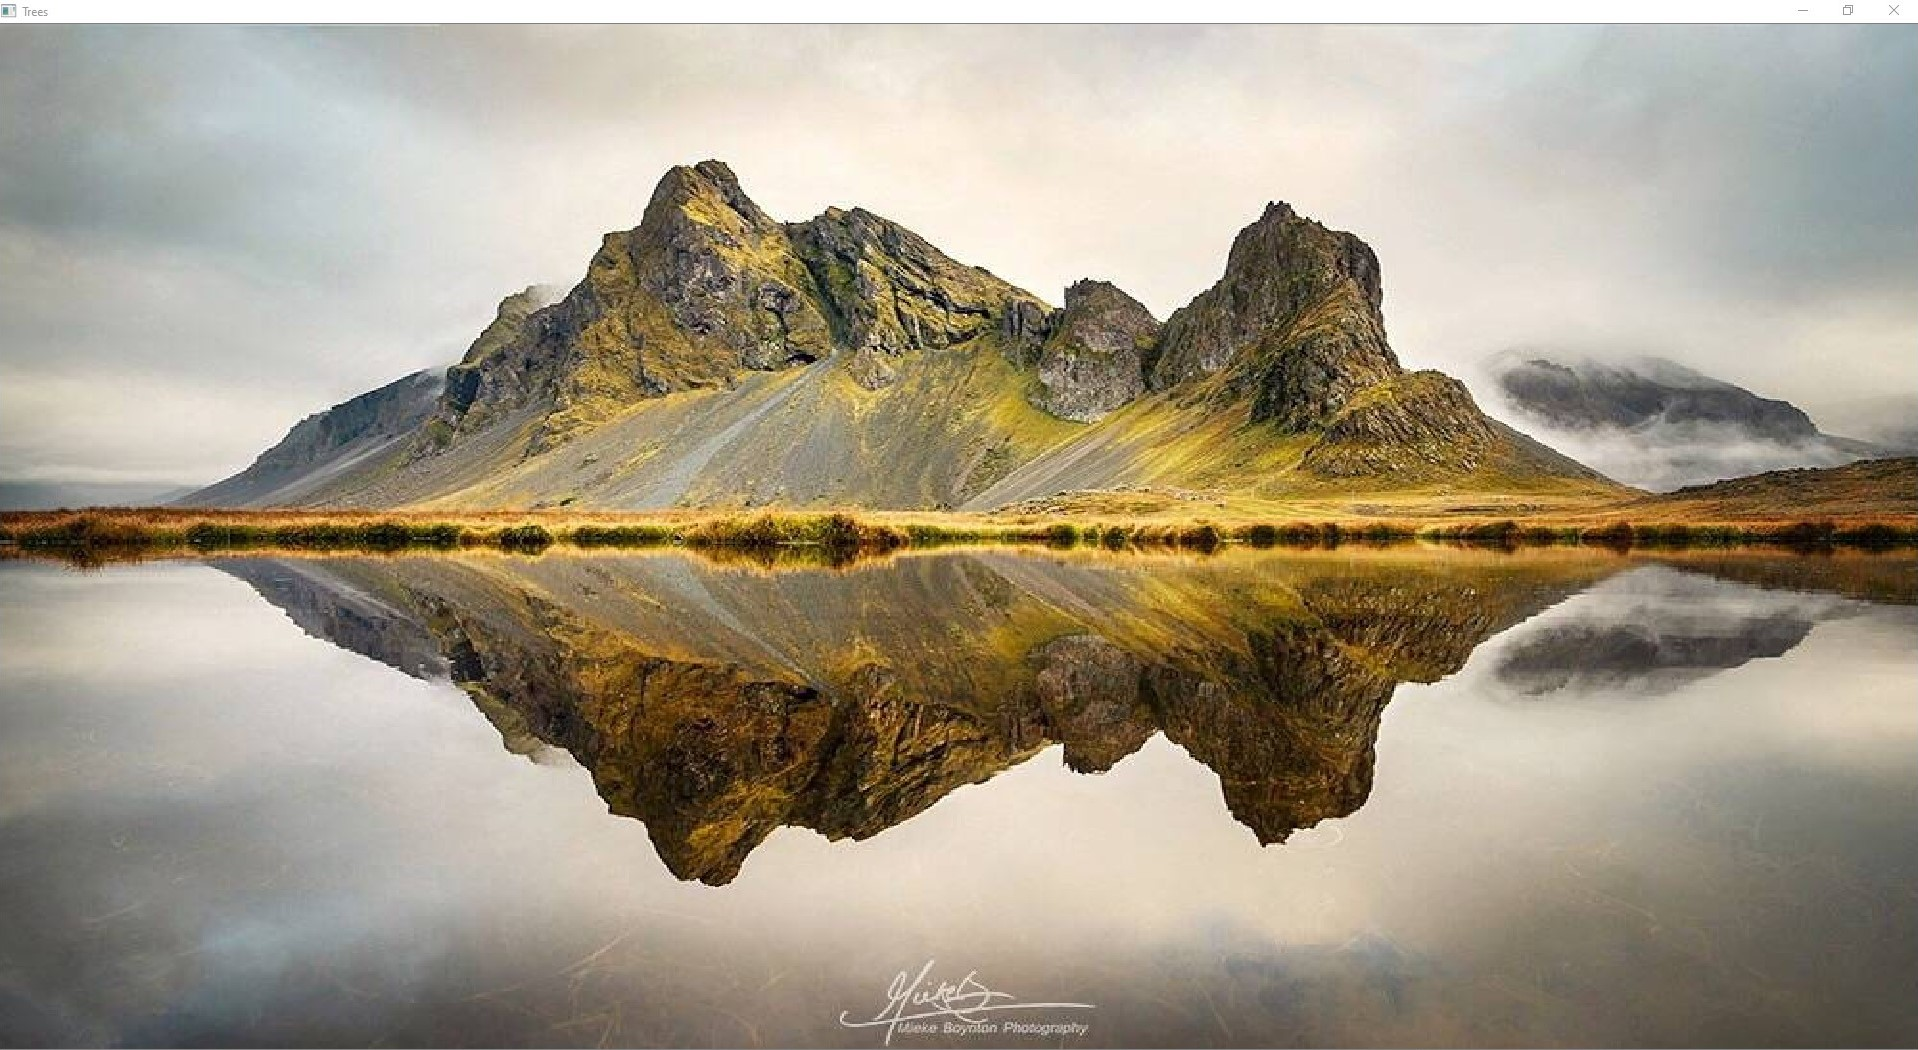
\includegraphics[width=1\textwidth]{images/b8}
\caption{\footnotesize{Figure\_8.jpg}}
\label{img:benchmark8}
\end{center}
\end{figure}

\begin{figure}[h]
\begin{center}
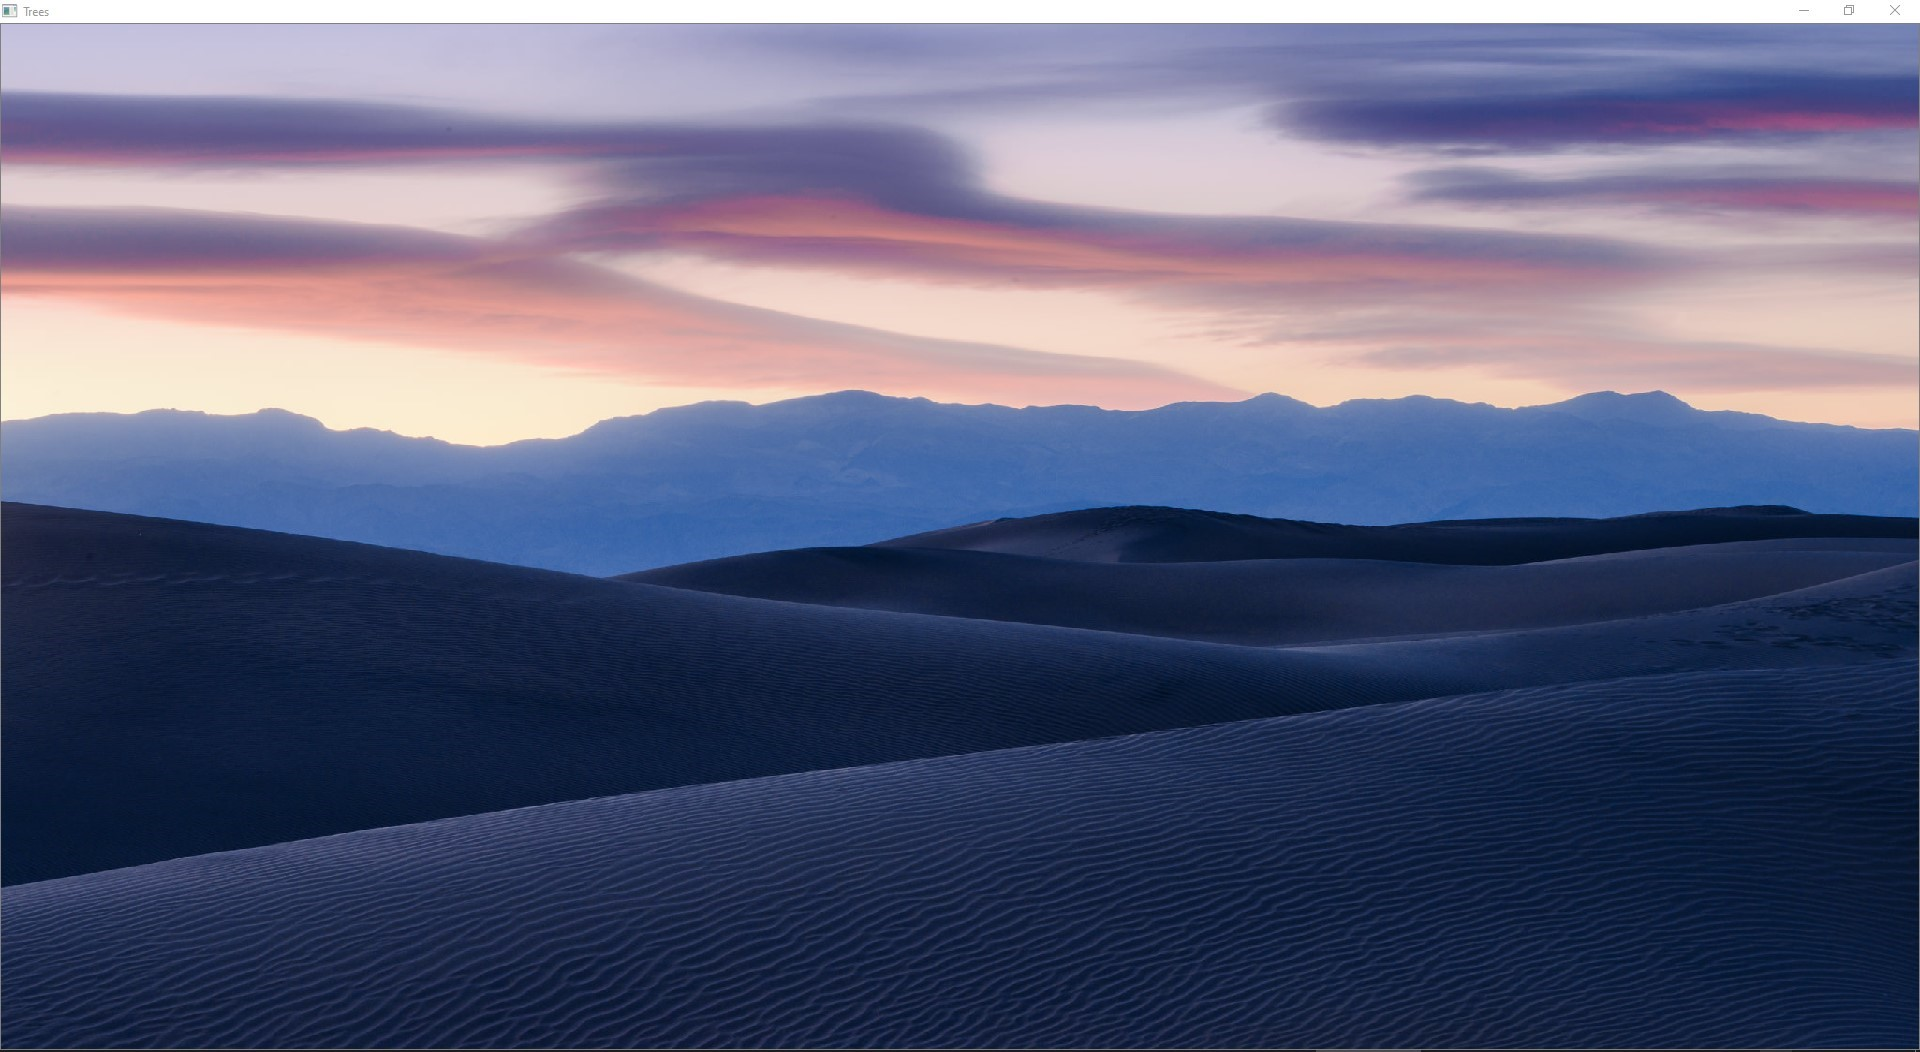
\includegraphics[width=1\textwidth]{images/b9}
\caption{\footnotesize{Figure\_9.jpg}}
\label{img:benchmark9}
\end{center}
\end{figure}

There were no false positives in figures \ref{img:benchmark7}, \ref{img:benchmark8} and \ref{img:benchmark9}, even implementing significant changes to the parameters. However, this is not always true.

\subsection{Training Dataset}
Some tests were performed on the training set, since the training phase did not cover the entire detection algorithm but just the creation of the BoW data required for classification. 

Figures \ref{img:train9} and \ref{img:train101} show a couple of false positives, both related to rocky features. In some conditions, in fact, the program interprets them as part of a tree.
Nevertheless, other rocky images are just fine (like \textit{Figure \ref{img:train102}}).

Figures \ref{img:train5}, \ref{img:train6} and \ref{img:trainb6} show other results.

\begin{figure}[h]
\begin{center}
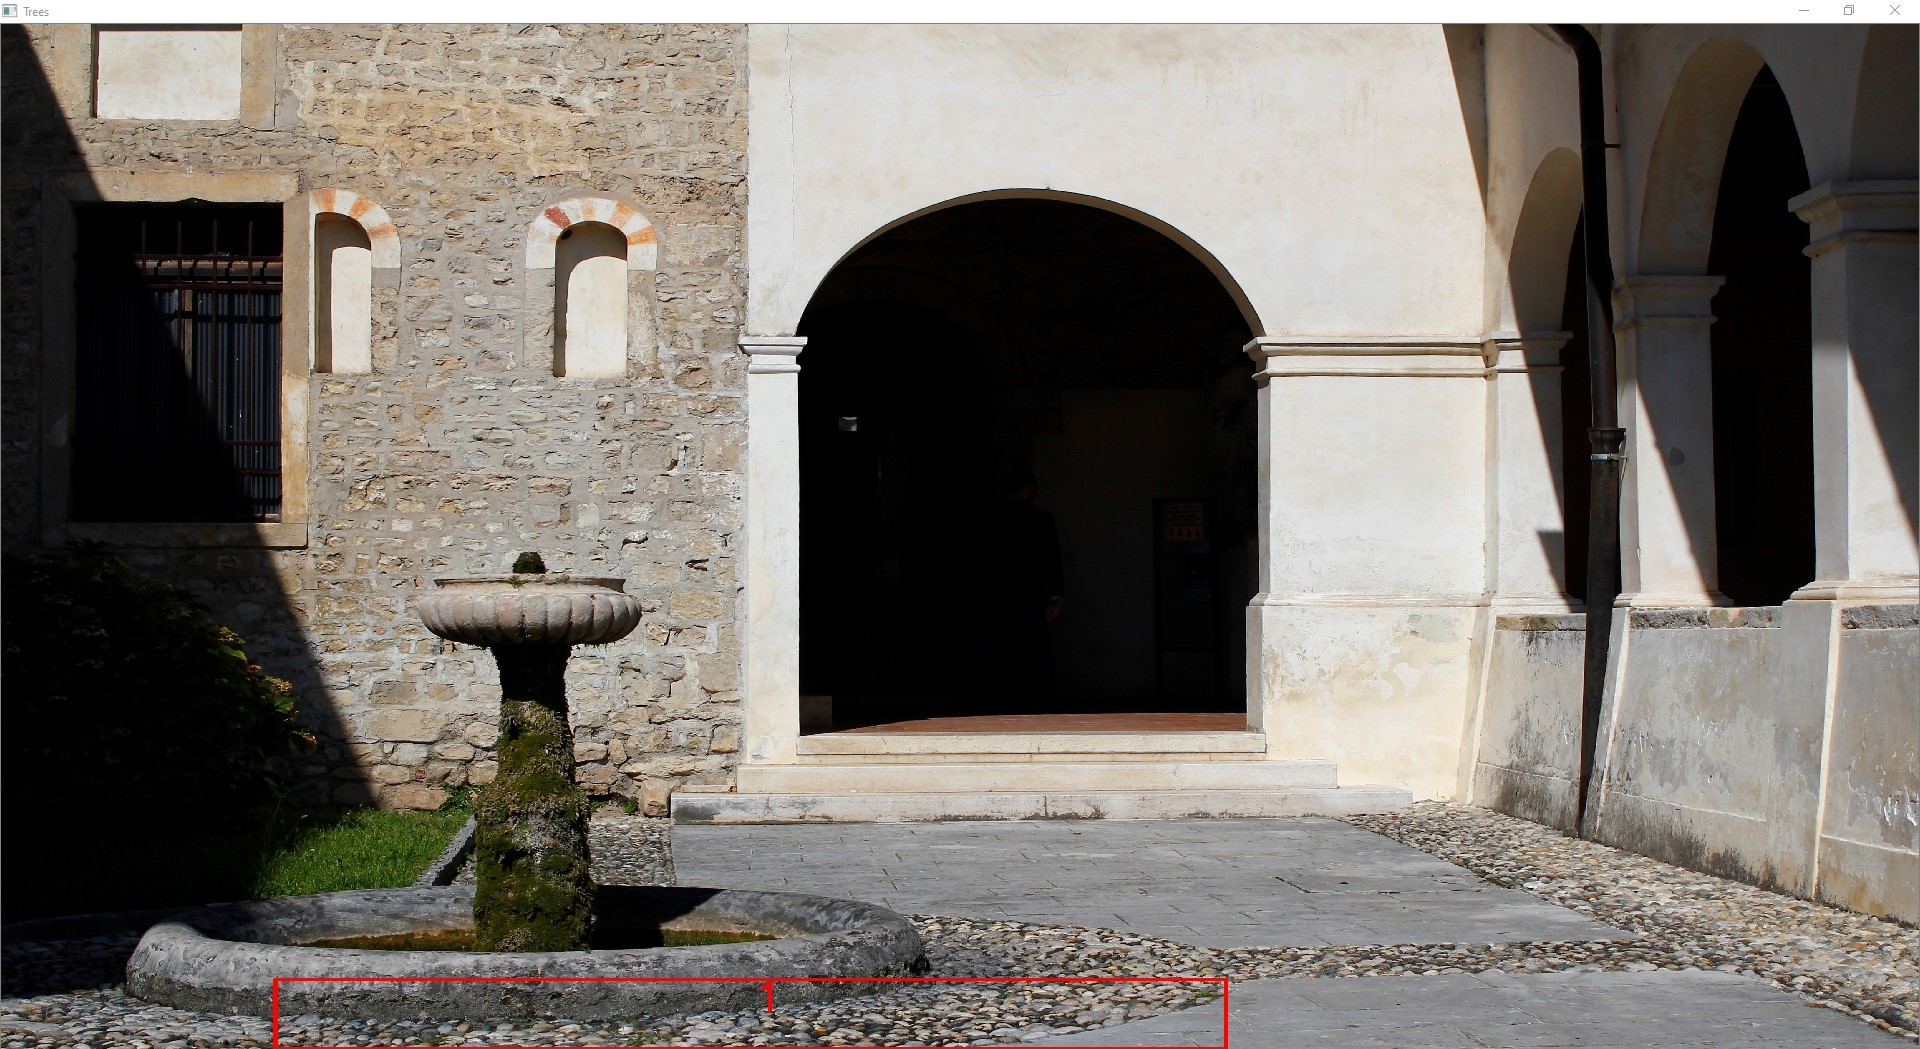
\includegraphics[width=1\textwidth]{images/train9}
\caption{\footnotesize{C\_9.jpg}}
\label{img:train9}
\end{center}
\end{figure}

\begin{figure}[h]
\begin{center}
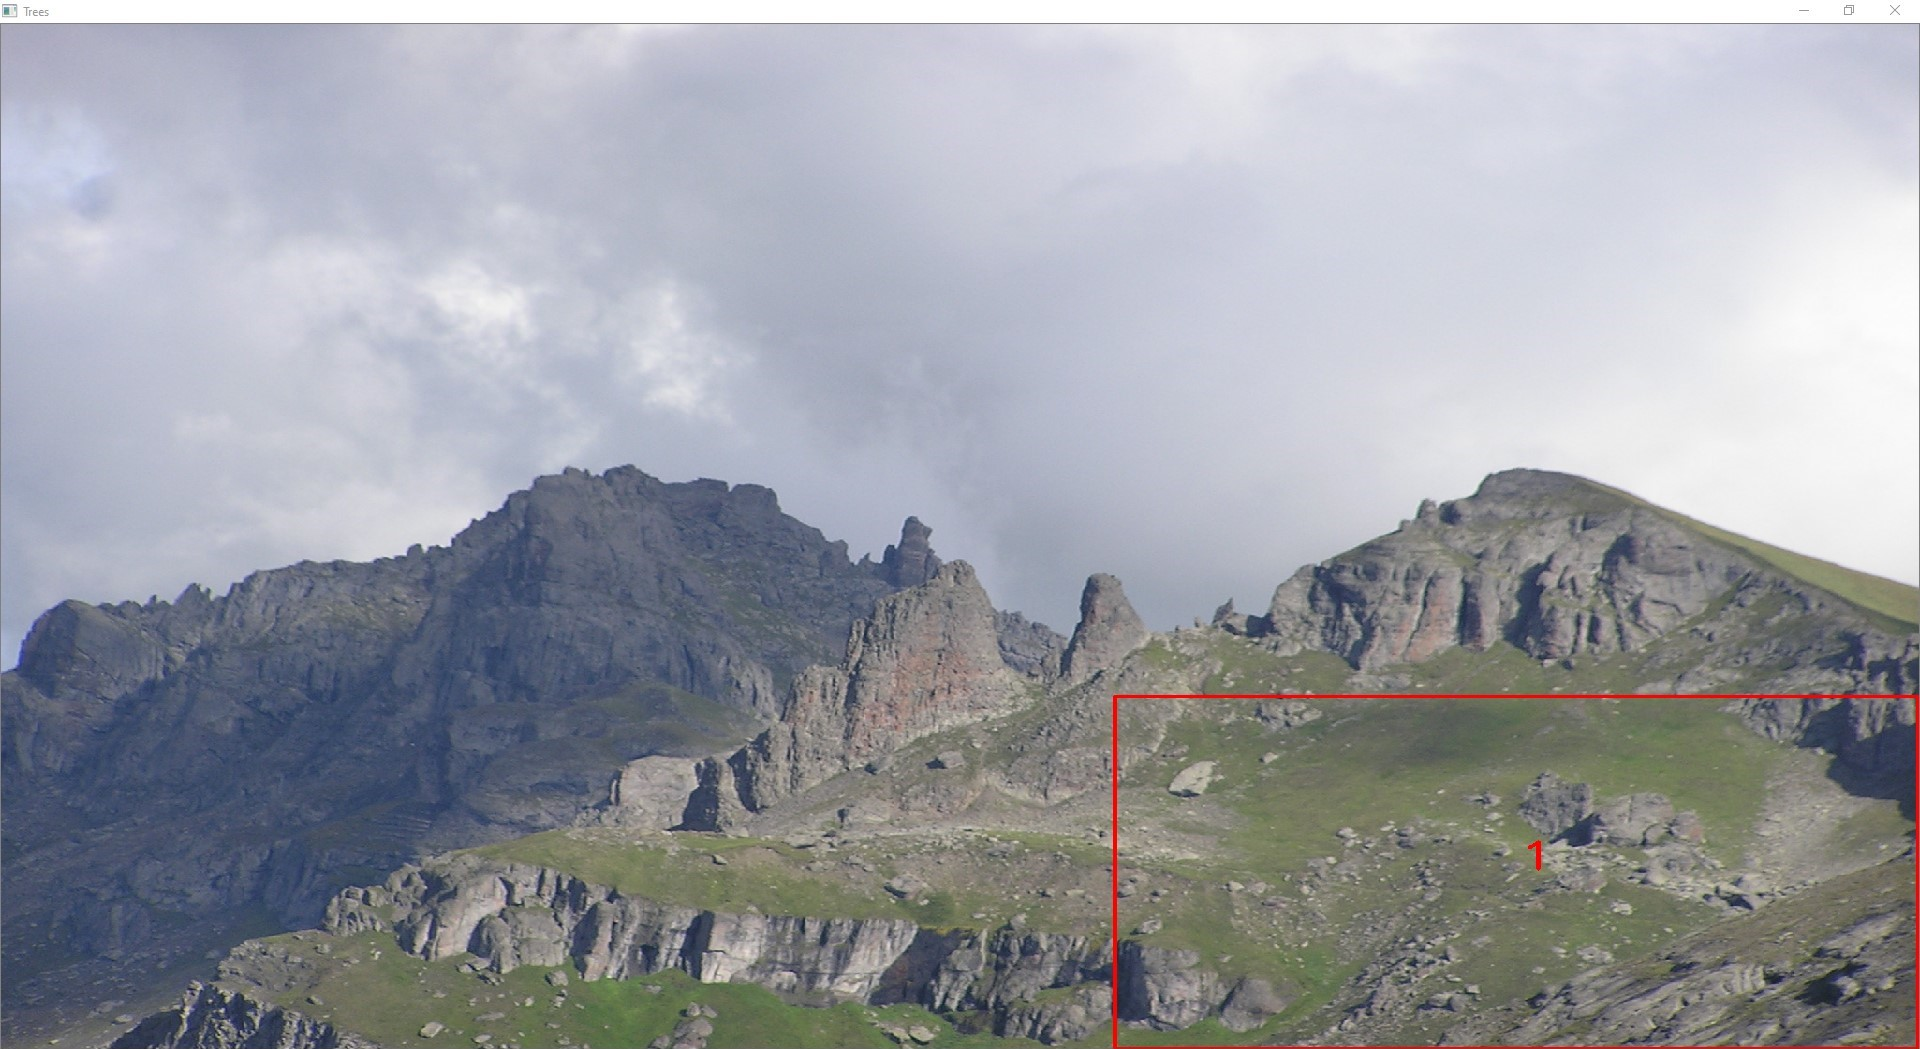
\includegraphics[width=1\textwidth]{images/train101}
\caption{\footnotesize{C\_101.jpg}}
\label{img:train101}
\end{center}
\end{figure}

\begin{figure}[h]
\begin{center}
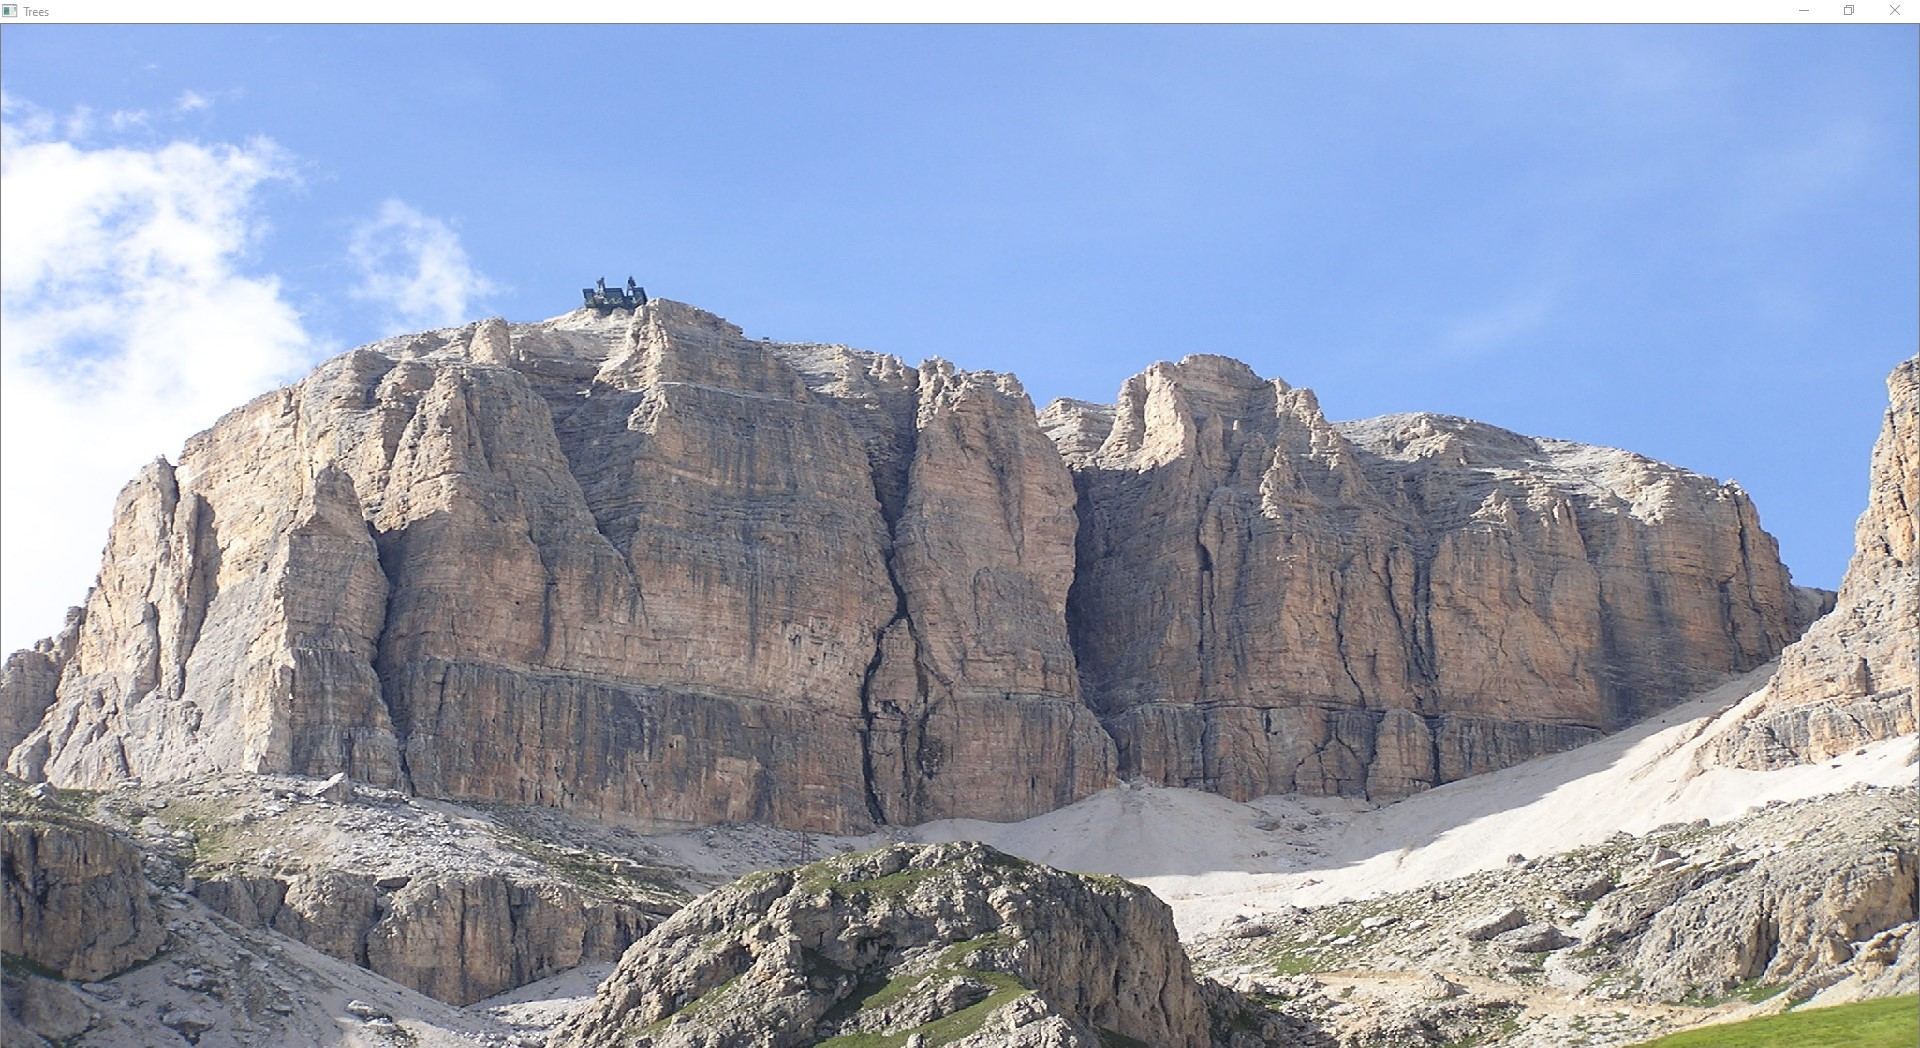
\includegraphics[width=1\textwidth]{images/train102}
\caption{\footnotesize{C\_102.jpg}}
\label{img:train102}
\end{center}
\end{figure}

\begin{figure}[h]
\begin{center}
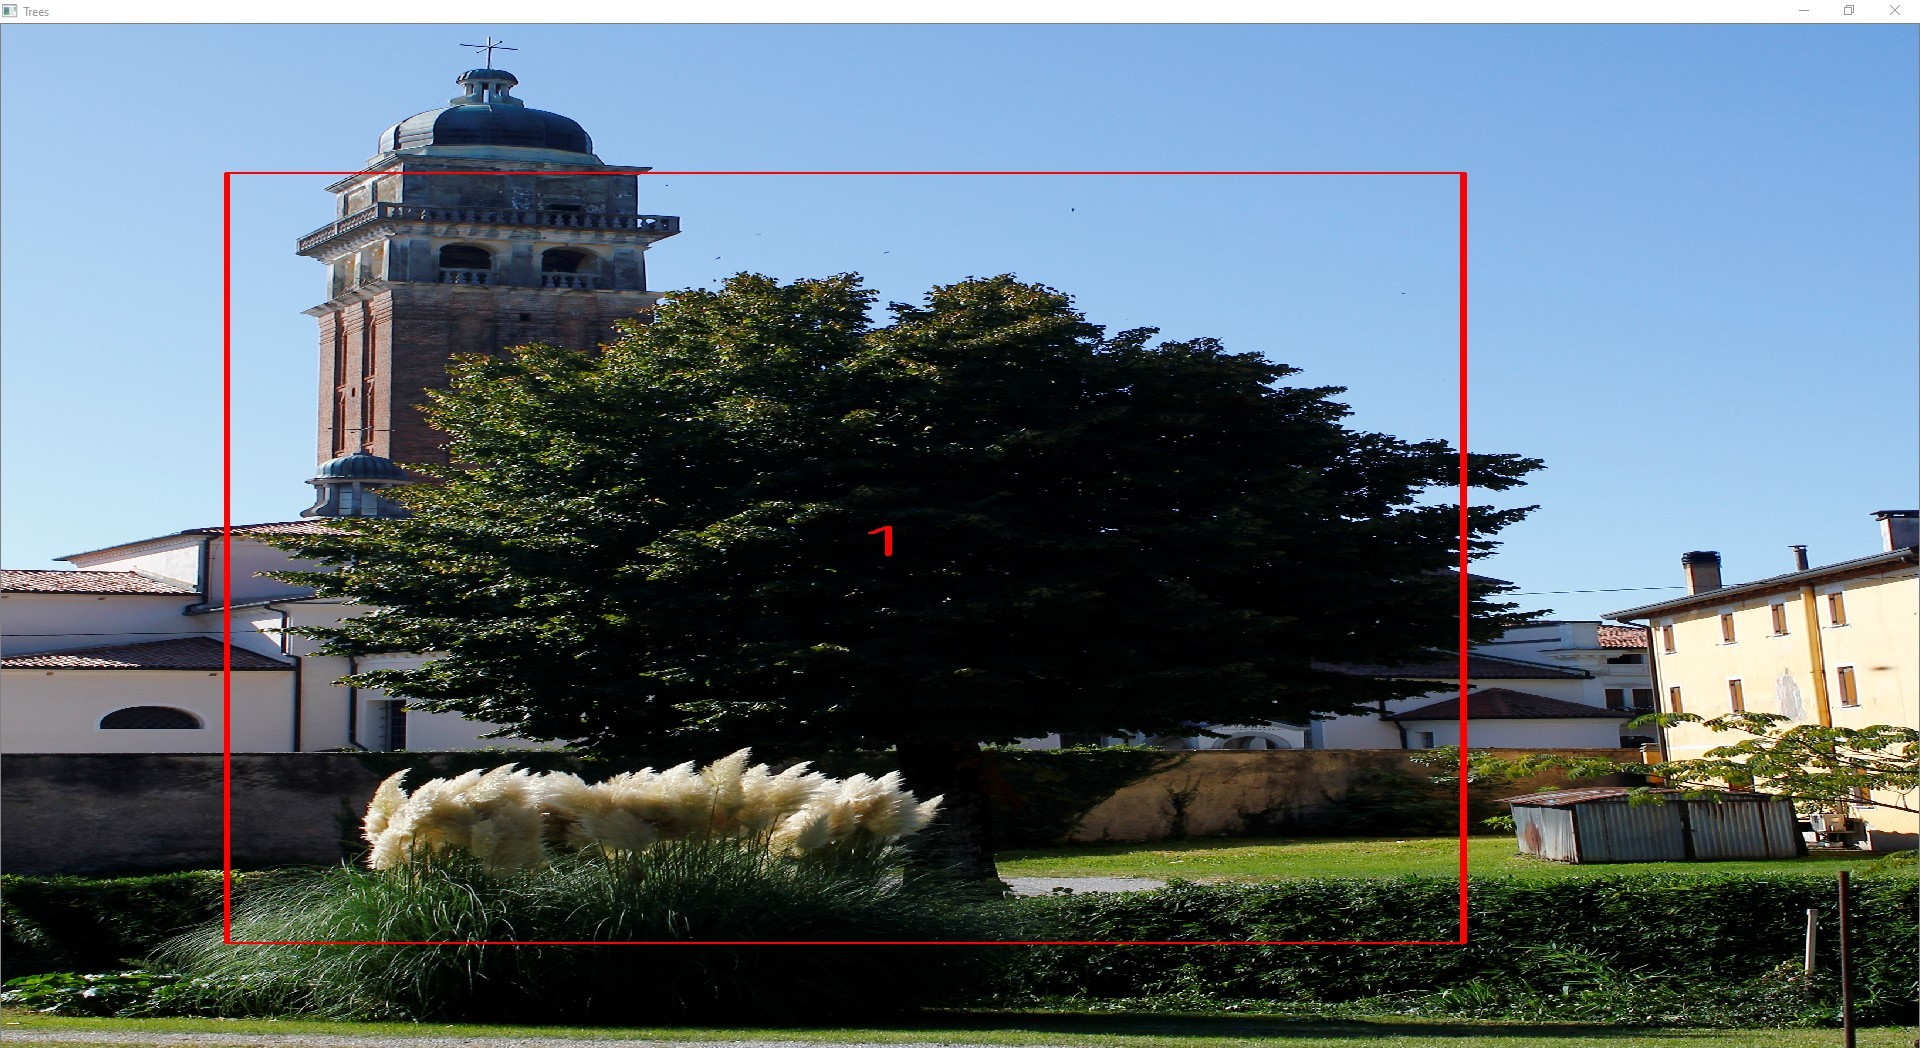
\includegraphics[width=1\textwidth]{images/train5}
\caption{\footnotesize{C\_5.jpg}}
\label{img:train5}
\end{center}
\end{figure}

\begin{figure}[h]
\begin{center}
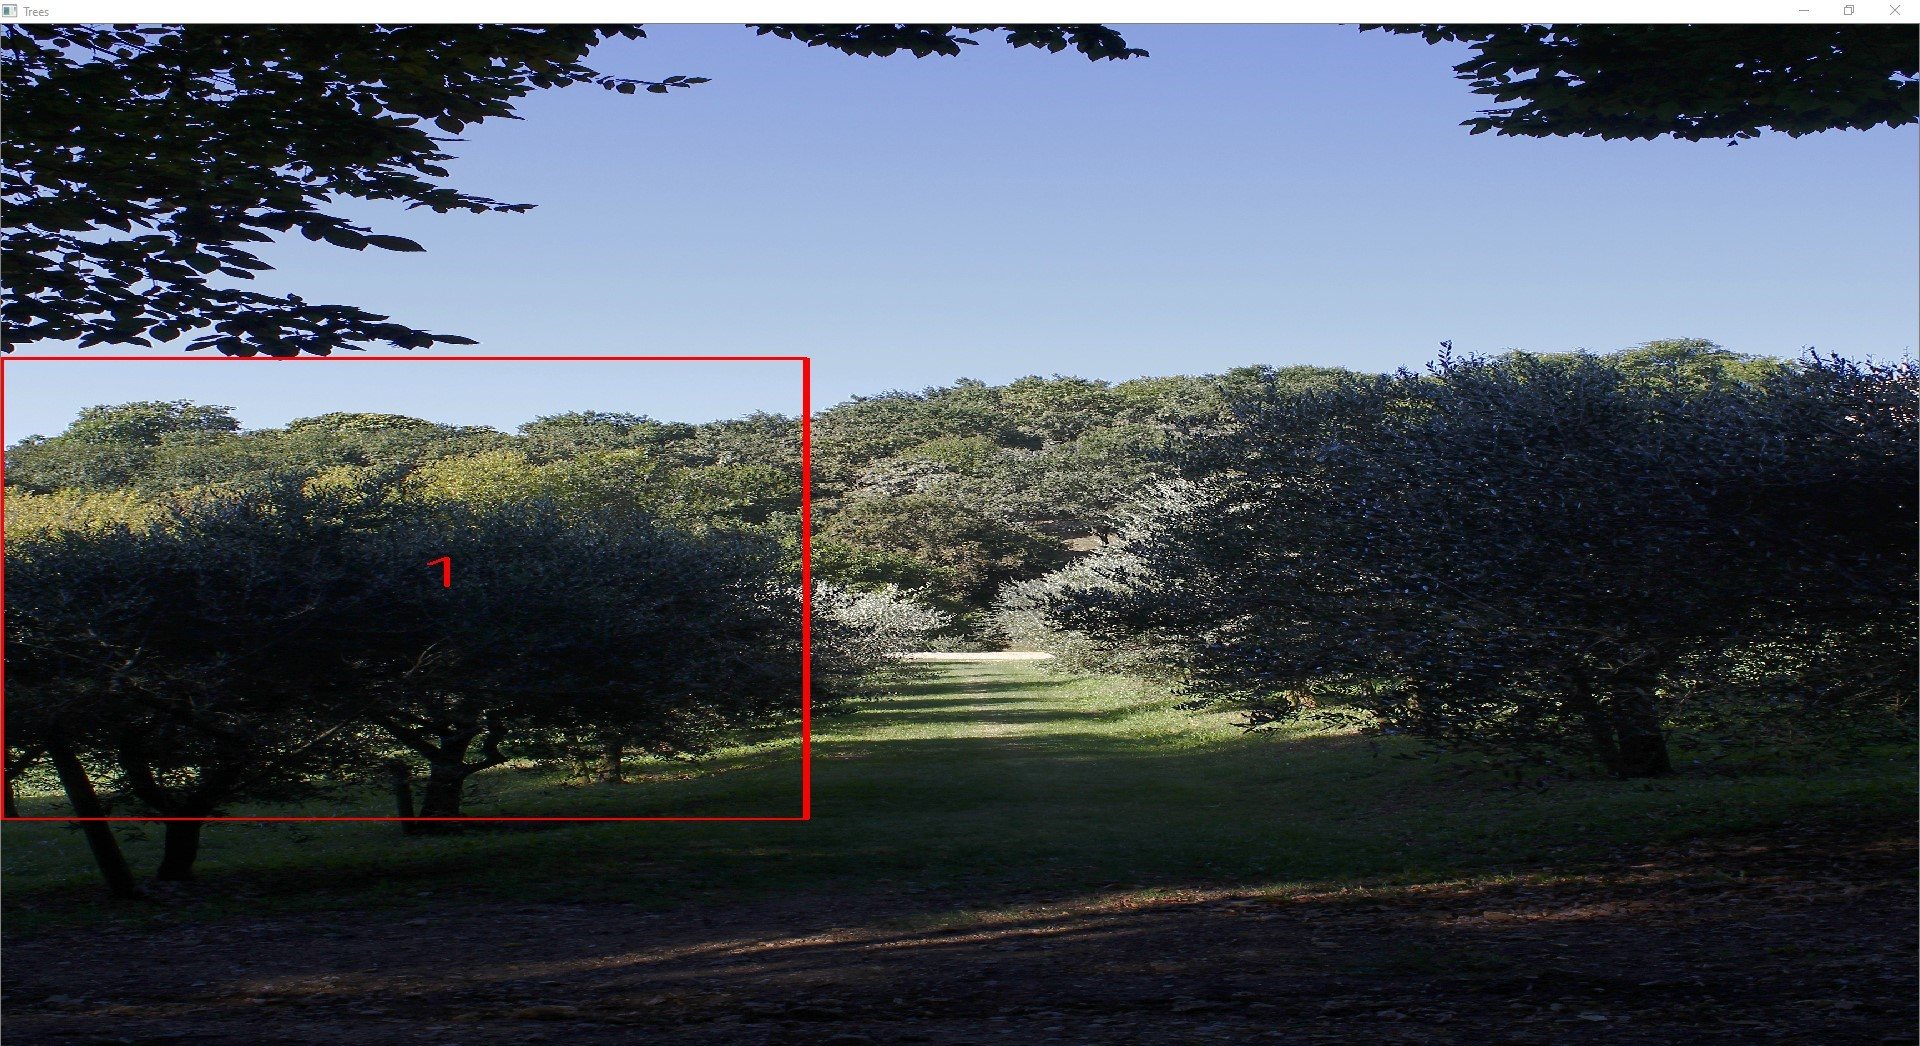
\includegraphics[width=1\textwidth]{images/train6}
\caption{\footnotesize{C\_6.jpg}}
\label{img:train6}
\end{center}
\end{figure}

\begin{figure}[h]
\begin{center}
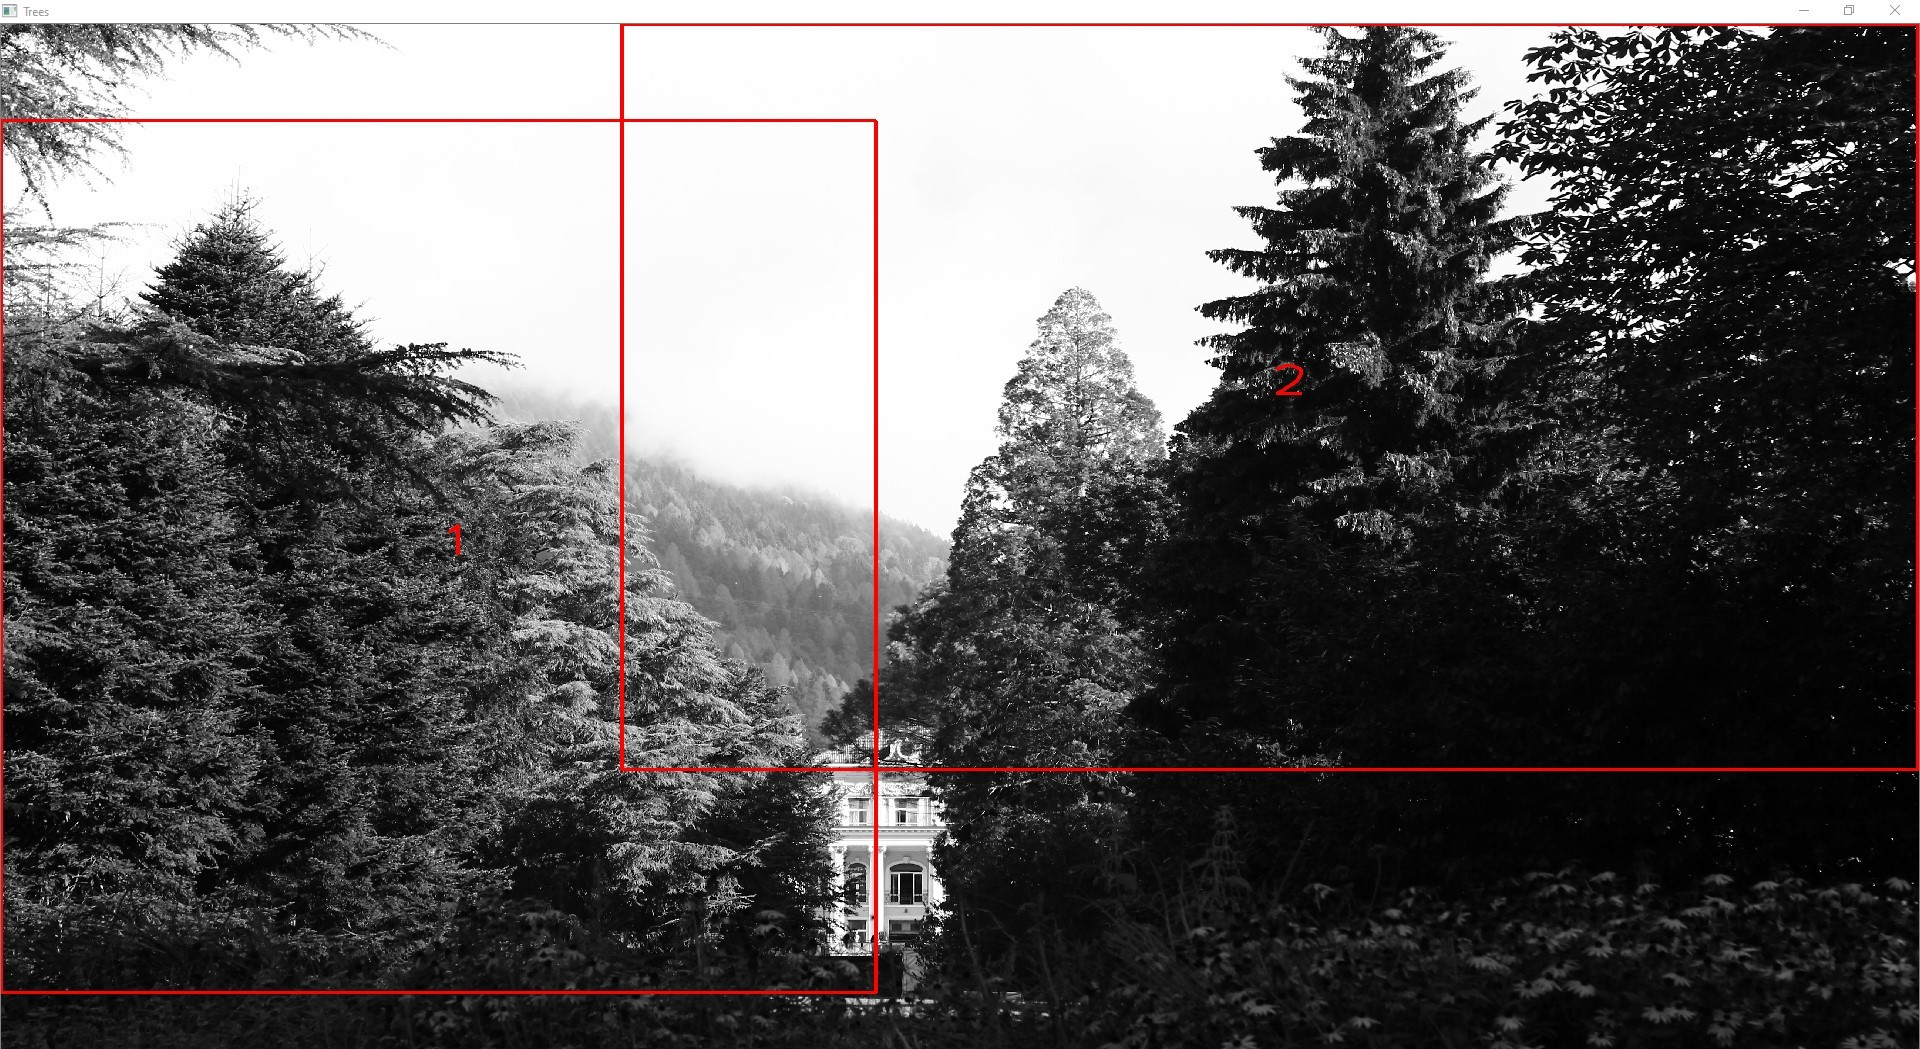
\includegraphics[width=1\textwidth]{images/trainb6}
\caption{\footnotesize{BW\_6.jpg}}
\label{img:trainb6}
\end{center}
\end{figure}


\end{document}